\documentclass[12pt,english]{article}

\usepackage{amsmath,amssymb,amsthm,epsfig,lineno,rotfloat,psfrag,natbib,caption,setspace,url,bm,geometry}
\usepackage{ecology}
\usepackage{graphicx}

\geometry{verbose,letterpaper,tmargin=2.54cm,bmargin=2.54cm,lmargin=2.54cm,rmargin=2.54cm}

%\setlength{\evensidemargin}{0in} \setlength{\oddsidemargin}{0in}
%\setlength{\topmargin}{-0.65in} \setlength{\textwidth}{6.5in}
%\setlength{\textheight}{9.5in} \setlength{\topskip}{0in}
%\setlength{\headheight}{0in}


%\newcommand{\yst}{\ensuremath{y_{st}}}
%\newcommand{\tyst}{\ensuremath{\tilde y_{st}}}
%\newcommand{\tzs}{\ensuremath{\tilde z_{s}}}
%\newcommand{\zs}{\ensuremath{z_{s}}}
%\newcommand{\bg}{\ensuremath{\boldsymbol{\gamma}}}
%\newcommand{\bxs}{\ensuremath{\mathbf{x}_{s}}}
%\newcommand{\bxst}{\ensuremath{\mathbf{x}_{st}}}
%\newcommand{\bK}{\ensuremath{\mathbf{K}}}
%\newcommand{\bn}{\ensuremath{\boldsymbol{\eta}}}
%\newcommand{\bb}{\ensuremath{\boldsymbol{\beta}}}
%\newcommand{\ba}{\ensuremath{\boldsymbol{\alpha}}}
%\newcommand{\by}{\ensuremath{\mathbf{y}}}
%\newcommand{\bz}{\ensuremath{\mathbf{z}}}
%\newcommand{\bX}{\ensuremath{\mathbf{X}}}
%\newcommand{\be}{\ensuremath{\boldsymbol{\epsilon}}}
%\newcommand{\bQ}{\ensuremath{\mathbf{Q}}}
%\newcommand{\bO}{\ensuremath{\boldsymbol{\Omega}}}
%\newcommand{\bm}{\ensuremath{\boldsymbol{\mu}}}




\bibpunct{(}{)}{,}{a}{}{;}

\bibliographystyle{ecology}
\raggedbottom


\captionsetup[table]{margin=0pt,font=small,labelfont={sc},justification=justified,labelsep=period}
\captionsetup[figure]{margin=0pt,font=small,labelfont={sc},justification=justified,labelsep=period,name=Fig}



\begin{document}
\begin{spacing}{1.9}

\begin{center}
On extrapolating past the range of observed data when making statistical predictions in ecology
\bigskip\\
\normalsize
{\sc Paul B. Conn$^{1,}$\footnotemark[2] and
Devin S. Johnson$^1$, Peter L. Boveng$^1$ }\smallskip\\
$^1${\em National Marine Mammal Laboratory, NOAA, National Marine Fisheries Service,
Alaska Fisheries Science Center, 7600 Sand Point Way NE, Seattle,
WA 98115 USA }\\ \medskip
\end{center}
\footnotetext[2]{Email: paul.conn@noaa.gov}


\raggedright \setlength{\parindent}{0.3in}
%\renewcommand{\baselinestretch}{1.8}\normalsize
\clubpenalty=0
 \linenumbers


{\em Abstract.\ } Ecologists are increasingly using statistical models to predict animal abundance and occurrence in unsampled locations. The reliability of such predictions depends on a number of factors, including sample size, how far prediction locations are from the observed data, and similarity of predictive covariates in locations where data are gathered to locations where predictions are desired.  In this paper, we propose extending Cook's notion of an independent variable hull (IVH), developed originally for application with linear regression models, to generalized regression models as a way to help assess the potential reliability of predictions in unsampled areas.  Predictions occurring inside the generalized independent variable hull (gIVH) can be regarded as interpolations, while predictions occurring outside the gIVH can be regarded as extrapolations worthy of additional investigation or skepticism. We conduct a simulation study to demonstrate the usefulness of this metric for limiting the scope of spatial inference when conducting model-based abundance estimation from survey counts.  In this case, limiting inference to the gIVH substantially reduces bias, especially when survey designs are spatially imbalanced.  We also demonstrate the utility of the gIVH in diagnosing problematic extrapolations when estimating the relative abundance of ribbon seals in the Bering Sea as a function of predictive covariates.  We suggest that ecologists routinely use diagnostics such as the gIVH and related metrics (e.g., prediction variance) to help gauge the reliability of predictions from statistical models.



{\em Key words: Abundance, Extrapolation, Independent Variable Hull, Prediction variance, Spatial regression, Species distribution model}

\centerline{\sc Introduction}


In ecology and conservation, a common goal is to make predictions about an unsampled random variable given a limited sample from the target population.  For instance, given a model ($\mathcal{M}$), estimated parameters ($\hat{\boldsymbol{\theta}}$), and a covariate vector ${\bf x}_i$, we often desire to predict a new observation $y_i$ at $i$ (where $i$ can be a design point or a spatial location).  For instance, we might use a generalized linear model \citep[GLM;][]{McCullaghNelder1989} or one of its extensions to predict species density or occurrence in a new location.  Such predictions can be of direct use to conservation and management, for instance, in estimating population abundance or distribution, and for projecting shifts in species range as a function of climate change. Spatially explicit estimates of abundance are also useful for testing theory related to biogeography or biodiversity \citep[e.g., neutral theory;][]{Hubbell2001}, and for accurately estimating the strength of density dependence \citep{ThorsonEtAlInPress}.

Early in their training, ecologists and statisticians are warned against extrapolating statistical relationships
past the range of observed data.  This caution is easily interpreted in the context of single-variable linear regression analysis; one should be cautious in using the fitted relationship to make predictions at some new response $y_i$ whenever $x_i < \min({\bf x})$ or $x_i > \max({\bf x})$ (where $x_i$ is an independent variable measured at point $i$).  But what about more complicated situations
where there are multiple explanatory variables, or when one uses a spatial regression model to account for the residual spatial autocorrelation that is inevitably present in patchy ecological data \citep{LichsteinEtAl2002}?  How reliable are spatially- or temporally-explicit predictions in sophisticated models for animal abundance and occurrence?

Statisticians have long struggled with the conditions under which fitted regression models are capable of
making robust predictions at new combinations of explanatory variables.  The issue is sometimes considered more of a
philosophical problem than a statistical one, and has even been likened to soothsaying \citep{EhrenbergBound1993}.  To our mind, the reliability of predictions from statistical models is likely a function of several factors, including (i) the intensity of sampling,
(ii) spatial or temporal proximity of the prediction location to locations where there are data, (iii) variability of the ecological process, and (iv) the similarity of explanatory covariates in prediction locations when compared to the ensemble of covariates for observed data locations.

Our aim in this paper is to investigate one possibility for defining extrapolation in the GLM and its extensions, including generalized additive models \citep[GAMs;][]{HastieTibshirani1999,Wood2006} and spatio-temporal regression models (STRMs).  In particular, we exploit some of the same ideas used in multiple linear regression regarding leverage and outliers \citep{Cook1979} to operationally define ``extrapolation" as making predictions that occur outside of a generalized independent variable hull (gIVH) of observed data points. Application of the gIVH and related criterion (e.g., prediction variance) can provide intuition regarding the reliability of predictions in unobserved locations, and can aid in model construction and survey design. We illustrate use of the gIVH on simulated count data, and on a species distribution model (SDM) for ribbon seals ({\it Histriophoca fasciata}) in the eastern Bering Sea.

\centerline{\sc GENERALIZING THE INDEPENDENT VARIABLE HULL}

Extrapolation is often distinguished from interpolation.  In a prediction context, we might define (admittedly quite imprecisely) that extrapolation consists of making predictions that are ``outside the range of observed data" while interpolation consists of making predictions ``inside the range of observed data."  But what exactly do we mean by ``outside the range of observed data"?  Predictions outside the range of observed covariates?  Predictions for locations that are so far from places where data are gathered that we are skeptical that the estimated statistical relationship still holds? To help guide our choice of an operational definition, we turn to early work on outlier detection in simple linear regression analysis.

In the context of outlier detection, Cook (\citeyear{Cook1979}) defined an independent variable hull (IVH) as the smallest convex set containing all design points of a full-rank linear regression model.  Linear regression models are often written in matrix form, i.e.,
\begin{linenomath*}
\begin{equation*}
  {\bf Y} = {\bf X} \boldsymbol{\beta} + \boldsymbol{\epsilon},
\end{equation*}
\end{linenomath*}
where ${\bf Y}$ are observed responses, ${\bf X}$ is a so-called design matrix that includes explanatory variables \citep[see e.g.,][]{Draper1966}, and $\boldsymbol{\epsilon}$ represent normally distributed residuals (here and throughout the paper, bold symbols will be used to denote vectors and matrices).
Under this formulation, the IVH is defined relative to the hat matrix, ${\bf V}_{\rm LR}={\bf X}({\bf X}^\prime{\bf X})^{-1}{\bf X}^\prime$ (where the subscript ``LR" denotes linear regression).  Letting $v$ denote the maximum diagonal element of ${\bf V}_{LR}$, one can examine whether a new design point, ${\bf x}_0$ is within the IVH.  In particular, ${\bf x}_0$ is within the IVH whenever
\begin{linenomath*}
\begin{equation}
  \label{eq:IVH}
  {\bf x}_0^\prime ({\bf X}^\prime{\bf X})^{-1}{\bf x}_0 \le v.
\end{equation}
\end{linenomath*}
Cook (\citeyear{Cook1979}) used this concept to identify influential observations and possible outliers, arguing that design points near the edge of the IVH are deserving of special attention.  Similarly, points outside the IVH should be interpreted with caution.

We simulated two sets of design data to help illustrate application of the IVH (Fig. \ref{fig:IVH}).  In simple linear regression with one predictor variable, predictions on a hypothetical response variable obtained at covariate values slightly outside the range of observed data are also outside the IVH.  However, fitting a quadratic model exhibits more nuance; if there is a large gap between design points, intermediate covariate values may also be outside of the IVH and thus more likely to result in problematic predictions.  Fitting a model with two covariates and both linear and quadratic effects, the shape of the IVH is somewhat more irregular, and even includes a hole in the middle of the surface when interactions are modeled (Fig. \ref{fig:IVH}).  These simple examples highlight the sometimes counterintuitive nature of predictive inference, a problem that can only become worse as models with more dimensions are contemplated (including those with temporal or spatial structure).  Fortunately, the ideas behind the IVH provide a potential way forward.

Cook's (1979) formulation for the IVH is particular to linear regression analysis, which assumes independent and identically distributed ($iid$) Gaussian error. Thus, it is not directly applicable to generalized models, such as those including alternative error distributions (e.g., Poisson, binomial) or spatial random effects.  Further, the hat matrix is not necessarily well defined for models with more general spatial structure. However, since the hat matrix is proportional to prediction variance, Cook (1979) notes that design points with maximum prediction variance will be located on the boundary of the IVH.  We therefore define a generalized independent variable hull (gIVH) as the set of all potential design points $\mathcal{S}_0$ (note that $\mathcal{S}_0$ can include both observed and unobserved design points) such that
\begin{linenomath*}
\begin{equation}
  \label{eq:gIVH}
  {\rm var}(\lambda_i) \le {\rm max} [{\rm var}(\boldsymbol{\lambda}_{\mathcal{S}})],
\end{equation}
\end{linenomath*}
where $i \in \mathcal{S}_0$, $\lambda_i$ corresponds to the mean prediction at $i$, $\mathcal{S}$ denotes the set of observed design points, and $\boldsymbol{\lambda}_\mathcal{S}$ denotes predictions at $\mathcal{S}$.

Generalizations of the linear model are often written in the form
\begin{linenomath*}
\begin{equation}
  Y_i \sim f_Y(g^{-1}(\mu_i)),
\end{equation}
\end{linenomath*}
where $f_Y$ denotes a probability density or mass function (e.g., Bernoulli, Poisson), $g$ gives a link function, and
$\mu_i$ is a linear predictor.  For many such generalizations, it is possible to specify the $\mu_i$ as
\begin{linenomath*}
\begin{equation}
  \boldsymbol{\mu} = {\bf X}_{aug}\boldsymbol{\beta}_{aug} + \boldsymbol{\epsilon},
  \label{eq:mu-aug}
\end{equation}
\end{linenomath*}
where the $\boldsymbol{\epsilon}$ represent Gaussian error, ${\bf X}_{aug}$ denotes an augmented design matrix, and $\boldsymbol{\beta}_{aug}$ denote an augmented vector of parameters.  For instance, in a spatial model, $\boldsymbol{\beta}_{aug}$ might include both fixed effect parameters and spatial random effects in a reduced dimension subspace (see Appendix A for examples of how numerous types of models can be written in this form).

When models are specified as in Eq. \ref{eq:mu-aug}, we can write prediction variance generically as
\begin{linenomath*}
\begin{equation}
  \label{eq:var-mu}
  {\rm var}(\boldsymbol{\mu}_x)= {\bf x} {\rm var}(\hat{\boldsymbol{\beta}}_{aug}) {\bf x}^\prime,
\end{equation}
\end{linenomath*}
where it is understood that the exact form of ${\bf x}$ and ${\rm var}(\hat{\boldsymbol{\beta}}_{aug})$ depends on the model chosen (i.e., GLM, GAM, or STRM; Appendix A). This expression for prediction variance is on the linear predictor scale; if a non-identity link function is used, we can use the delta method \citep{Dorfman1938,VerHoef2012b} to approximate prediction variance on the real scale (i.e., the scale in which data are measured; see Appendix A).  Unlike Cook's original formulation, the gIVH will often involve unknown parameters.  For most of the following treatment, we shall assume that data have already been collected (see Discussion for comments on the potential use of the gIVH in survey planning), and that informative probability distributions can be specified for these parameters.

We propose to use the gIVH in much the same manner as Cook (1979).  In particular, we use the gIVH to differentiate whether spatial predictions are interpolations (predictive design points lying inside the gIVH) or extrapolations (predictive design points lying outside the gIVH).  The gIVH, together with posterior prediction variance, seem ideally suited to diagnosing potential extrapolation issues. Further, one can compare prediction variance in places one has data to places where predictions are desired to gauge the relative amount of information that predictions will be based on.

\subsection{Computing}

We developed a package \texttt{SpatPred} in the R statistical programming environment \citep{RTeam2012} to simulate data and conduct all analyses.  The seal dataset is included as part of this package, and is available at \url{https://github.com/pconn/SpatPred}.  The R package has also been archived via figshare [WE PLAN TO DO THIS WHEN THE MANUSCRIPT IS ACCEPTED FOR PUBLICATION].


\centerline{\sc Examples}

\subsection{Simulation study}


We conducted a simulation study to investigate whether the gIVH (and accompanying prediction variance) was useful in diagnosing prediction biases when analyzing animal count data. For each of 100 simulations, we generated animal abundance over a $30 \times 30$ grid assuming that animal density was homogeneous in each grid cell.  Animal abundance was generated as a function of three hypothetical spatially autocorrelated habitat covariates (Appendix B).   For each simulated landscape, we conducted virtual surveys of $n=45$ survey units using two different designs: (1) a spatially balanced sample \citep{StevensOlsen2004}, and (2) a convenience sample where the probability of sampling was greater for cells closer to a ``base of operations" located in the middle of the survey grid. The former approach preserves randomness while seeking a degree of regularity when distributing sampling locations across the landscape, while the latter may be easier to implement logistically.

We configured virtual sampling quadrats such that they encompassed 10\% of the area of each selected grid cell.  For ease of presentation and analysis, we assumed detection probability was 100\% in each quadrat.  Once animal counts were simulated, three different estimation models were fitted to the data: a GLM, a GAM, and an STRM (Appendix A).  The fixed effects components of the GLM and STRM were configured to have both linear and quadratic covariate effects and first-order interactions, while the GAM expressed log-density as a function of smooth terms for each covariate (Appendix B).  Each model was provided with two of the three covariates used to generate the data.

For each simulated data set and model structure, we calculated the posterior predictive variance and resulting $\text{gIVH}$ as in Eq. \ref{eq:gIVH}. We then calculated posterior predictions of animal abundance within and outside of each gIVH in order to gauge bias as a function of this restriction.  Specifically, the performance of $\text{gIVH}$ may help decide its utility in limiting the scope of inference once data have been collected and analyzed, and perhaps point out areas worthy of additional sampling.  A fuller, technical description of the simulation study design and several illustrations are provided in Appendix B.

Posterior predictions from simulations indicated that the distribution for proportional error in total abundance was right skewed when statistical inference was made with regard to the entire survey area (Fig. B3).  This was particularly true for GLM and STRM models, and was exacerbated when convenience sampling was employed.  The magnitude of mean absolute bias was reduced when inference was constrained to the gIVH for all 6 configurations of survey design and estimation model.  For GLMs and STRMs, positive proportional bias was the rule, and was of concerning magnitude ($\approx 0.3$) for GLMs and STRMs when convenience sampling was employed and inference was not restricted to the gIVH.  By contrast, proportional bias was close to zero when inference was restricted to the gIVH.  Interestingly, the radial basis GAMs we employed often underestimated total abundance, perhaps because of dampening ``edge effects" at extreme ranges of observed covariates, or possibly because interactions among covariates were not modeled.


\subsection{Ribbon seal SDM}

To demonstrate application of the gIVH on a real dataset, we consider the case of estimating ribbon seal relative abundance from count data obtained during aerial surveys of the Bering Sea in April, 2012 (Fig. \ref{fig:flights}).  In this case, we wish to model seal counts as a function of habitat covariates and possible spatial autocorrelation, and to use predictions from this fitted model to estimate relative abundance for the entire study area.  For further background and details on these data, we refer the reader to Appendix C.

Inspection of ribbon seal data (Fig. \ref{fig:flights}) immediately reveals a potential
issue with spatial prediction: abundance of ribbon seals appears to be maximized in the southern and/or southeast quadrant of the surveyed area.  Predicting abundance in areas further south and east may thus prove problematic, as the values of several explanatory covariates (Fig. C1) are also maximized in these regions.  To illustrate, let $Y_i$ denote the ribbon seal count ($Y_i$) obtained in sampled grid cell $i$.  Suppose that counts arise according to a log-Gaussian Cox process, such that
\begin{eqnarray}
  \label{eqn:Cox}
  Y_i \sim {\rm Poisson}(\lambda_i) \mbox{ and } \\
  \log(\lambda_i) = \log(P_i) + \log(A_i) + \theta_i + \epsilon_i, \nonumber
\end{eqnarray}
where $P_i$ gives the proportion of area surveyed in grid cell $i$, $A_i$ gives the proportion of cell $i$ that is seal habitat, $\theta_i$ is a linear predictor, and $\epsilon_i$ is normally distributed $iid$ error.  By formulating $\theta_i$ differently, we can arrive at representations characteristic of GLMs, GAMs, and STRMs (see Appendix A).

We start by fitting a hierarchical GLM, GAM, and STRM to the full suite of predictor covariates (Fig. C1).  For the GLM and STRM, we fit a model with linear effects of all predictor variables and an additional quadratic term for ice concentration \citep[seal density is often maximized at an intermediate value of ice concentration; see][]{VerHoef2013,ConnEtAl2014}. For the GAM, smooth effects were included for each covariate, with 8 knots each.  As with simulated data examples, we adopted a Bayesian perspective and conducted estimation and posterior prediction using MCMC (see Appendix A for estimation algorithm details and Appendix C for further numerical details related to the ribbon seal example).

Initial spatial predictions using the three models (GLM, GAM, STRM) all produced extremely high, unbelievable predictions along the southern boundary of the study area (Fig. \ref{fig:ribbon_plot}).  Predictions in this region were also largely out of the gIVH, indicating the potential utility for the gIVH in revealing problematic extrapolations.
We considered several possible alternatives for trying to obtain more robust abundance estimates before settling on a preferred alternative.  First, one could refine the study area to eliminate predictions outside of the gIVH (as in the simulation study).  However, this is not ideal in that one does not get an abundance estimate for the whole study area, and it may be difficult to compare abundance from one year to the next using this approach. Second, one could consider a simpler estimation model, such as one post-stratifying by ecoregion \citep[as in][]{ConnEtAl2014}.  Finally, one could build in a priori knowledge of habitat preferences into the model structure.  We adopted the latter solution, incorporating ``pseudo-absences" (i.e., zero counts where sampling was not conducted) in locations where it would have been (nearly) impossible to detect seals.  Specifically, we inserted pseudo-absences in cells where ice concentrations were $<0.1\%$.  This solution seemed the most logical, as many of the large, anomalous predictions were over open water along the southern edge of the study area, where we would have obtained zero counts had they been surveyed.  This approach effectively requires that sea ice concentration be included as a predictive covariate to help model absences in cells without ice.

Fitting our three models to the augmented dataset with pseudo-absences, most predictions occurred within the gIVH (Fig. \ref{fig:ribbon_plot}).  The largest difference among the three models was in the southwest corner of the study area, coinciding with the few cells that were outside the gIVH in the three models.  Posterior summaries of abundance across the study area were very comparable (albeit with a longer right hand tail for the STRM), with $5\%$, $50\%$, and $95\%$ posterior prediction quantiles as follows: GLM (48686,64836,93927); GAM(46120,61214,90873); STRM(41039,63717,194095).  We note that these estimates are for example illustration only, as they are uncorrected for imperfect detection \citep[e.g., incomplete detection of thermal cameras, animals that were unavailable for sampling because they were in the water, species misidentification; see][]{ConnEtAl2014}.  Our approach here was to examine extrapolation and prediction error using relatively simple models, with the understanding that such effects are also likely to occur in complex models with more realistic observation processes.


\centerline{\sc Discussion}

We have demonstrated the capacity for certain classes of statistical models to produce biased predictions of animal abundance when extrapolating past the range of observed data.  In simulations, commonly used models (GLMs, STRMs) exhibited positive bias when predictions were required for the entire study area, particularly when convenience sampling was employed (with mean proportional bias $\approx 30\%$). In the ribbon seal example, naive extrapolation of fitted statistical relationships produced high positive bias along the southern boundary of the study area.  However, the gIVH appeared useful in diagnosing places where extrapolations from the fitted statistical model were problematic.  For instance, in the simulation study, limiting the scope of inference to locations falling within the gIVH reduced or eliminated bias.  For ribbon seal relative abundance, it was useful for confirming that the naive models needed to be reformulated, and that reformulated models (with pseudo-absence data) produced predictions in unsurveyed areas that were largely within the realm of observed data.

Our intent in writing this paper is to raise awareness of potential problems with extrapolation bias in statistical models, and to provide an additional tool (the gIVH) to help diagnose its presence.  Other approaches for selecting models to reduce overfitting, such as cross validation \citep[e.g.,][]{PicardCook1984}, are also useful for this purpose, but may not entirely eliminate the problem (particularly for sparse datasets). In fields such as species distribution modeling and model-based abundance estimation, the goal for analysts is often to build predictive maps of species abundance and/or occurrence using a limited number of sample locations.
In such applications, the ultimate aim of analysts should be to build models that have low bias and maximal precision.  However, traditional approaches to quantifying bias (e.g., goodness-of-fit statistics) only work with observed data points.  When inference is extended to unsampled locations, the gIVH appears to be a useful diagnostic for whether bias for predictions in unsampled locations can be expected.  In some cases, biological knowledge and intuition may be sufficient to diagnose anomalous predictions.  However, such determinations are likely to be quite subjective, and may prove insufficient when there are a large number of regression coefficients and interaction terms.  For instance, even relatively simple regression models may exhibit non-intuitive patterns (e.g., Fig. \ref{fig:IVH}).  Further, relying on expert opinion alone in successive rounds of model formulation and fitting may lead to investigators choosing models based on how much they like the results, which is clearly not ideal scientific practice.

The analyses in this paper focused on abundance estimation, which is necessarily non-negative.  As such, counts are usually analyzed with a log link function, and there is a much greater potential for positive bias than negative.  However, one could also apply the gIVH when predicting species occurrence from presence/absence data.  In this case, common link functions (e.g., probit or logit) are symmetric, and potential for positive and negative bias in predictive maps seem equally likely.  Future research should be directed to examine conditions under which the gIVH is a useful diagnostic in such applications.

One area that gIVH ideas may also prove useful is in formulating survey designs.  The topic of optimal (or near-optimal) spatial design has received considerable attention in the statistical literature, often in the context of designing environmental monitoring systems \citep{Muller2007}.  Optimal designs can be sensitive to the structure of the estimation model that is used, so that tailoring a survey design to a particular model can be somewhat dangerous if there is uncertainty about the ultimate ``best" structure for the model used to relate animal abundance and occurrence to available covariates.  Nevertheless, one could still think about augmenting a spatially balanced sampling design with a number of locations which are known or thought to have high prediction variance as a function of available covariates.  We are excited about this prospect, and it is a subject of current research.


\bibliography{master_bib}

\centerline{\sc Supplemental Material}

\centerline{\bf Appendix A}
Model formulation, Gibbs sampling algorithms, and gIVH calculations for certain classes and extensions of the generalized linear model ({\it Ecological Archives} XXXX-XXX-A1).

\centerline{\bf Appendix B}
Full details of simulation study examining predictive extrapolation ({\it Ecological Archives} XXXX-XXX-A2).

\centerline{\bf Appendix C}
Additional details on ribbon seal count data ({\it Ecological Archives} XXXX-XXX-A3).

\clearpage
%FIGURE 1. A ribbon seal, {\it Phoca fasciata}; the focus of spatial %modeling efforts in this paper.

FIGURE 1. Example IVHs constructed from simulated data.  In (A) and (B), linear regression is used to relate a response variable to a single covariate, $x$, obtained at locations denoted with an ``x".  Using $x$ as a simple linear effect (A), only predictions less than the minimum observed value of $x$ or greater than the maximum value of $x$ are outside the IVH (shaded area), as scaled prediction variance in these areas (solid line) is greater than the maximum scaled prediction variance for observed data (dashed line).  Using both linear and quadratic effects (B), some intermediate points are also outside the IVH.  When both linear and quadratic effects of two covariates ($x_1$ and $x_2$) are modeled, the IVH is more nuanced and depends on whether interactions are omitted (C) or included (D).


FIGURE 2. Aerial survey tracks over the Bering Sea, April 22-29, 2012 (blue lines) overlayed on a tesselated study area consisting of 25km by 25km grid cells (gray lines).  Dark gray indicates land, while the brown line indicates a 1000m depth contour, and the orange line shows the U.S Exclusive Economic Zone (EEZ) boundary. Colored pixels indicate ribbon seal counts along aerial transects. The average effective area surveyed in each grid cell was approximately $2.6km^2$ ($0.4\%$).  Note that surveys were designed to target multiple seal species, several of which had high densities further north (results not shown).

FIGURE 3.  Posterior mean predictions of ribbon seal apparent abundance across the eastern Bering sea from models fit to survey data.  Each row gives result for different model types (GLM, GAM, or STRM, respectively); left column plots give results for naive runs without pseudo-absences, while plots in the right column give predictions for runs where psuedo-absence data (i.e., 0 counts in cells with less than $0.1\%$ ice) were included. Cells highlighted in black indicate those where predictions were outside the generalized independent variable hull (gIVH).

\clearpage
\centerline{\sc Figures}



%\begin{figure}[!h]
%\begin{center}
%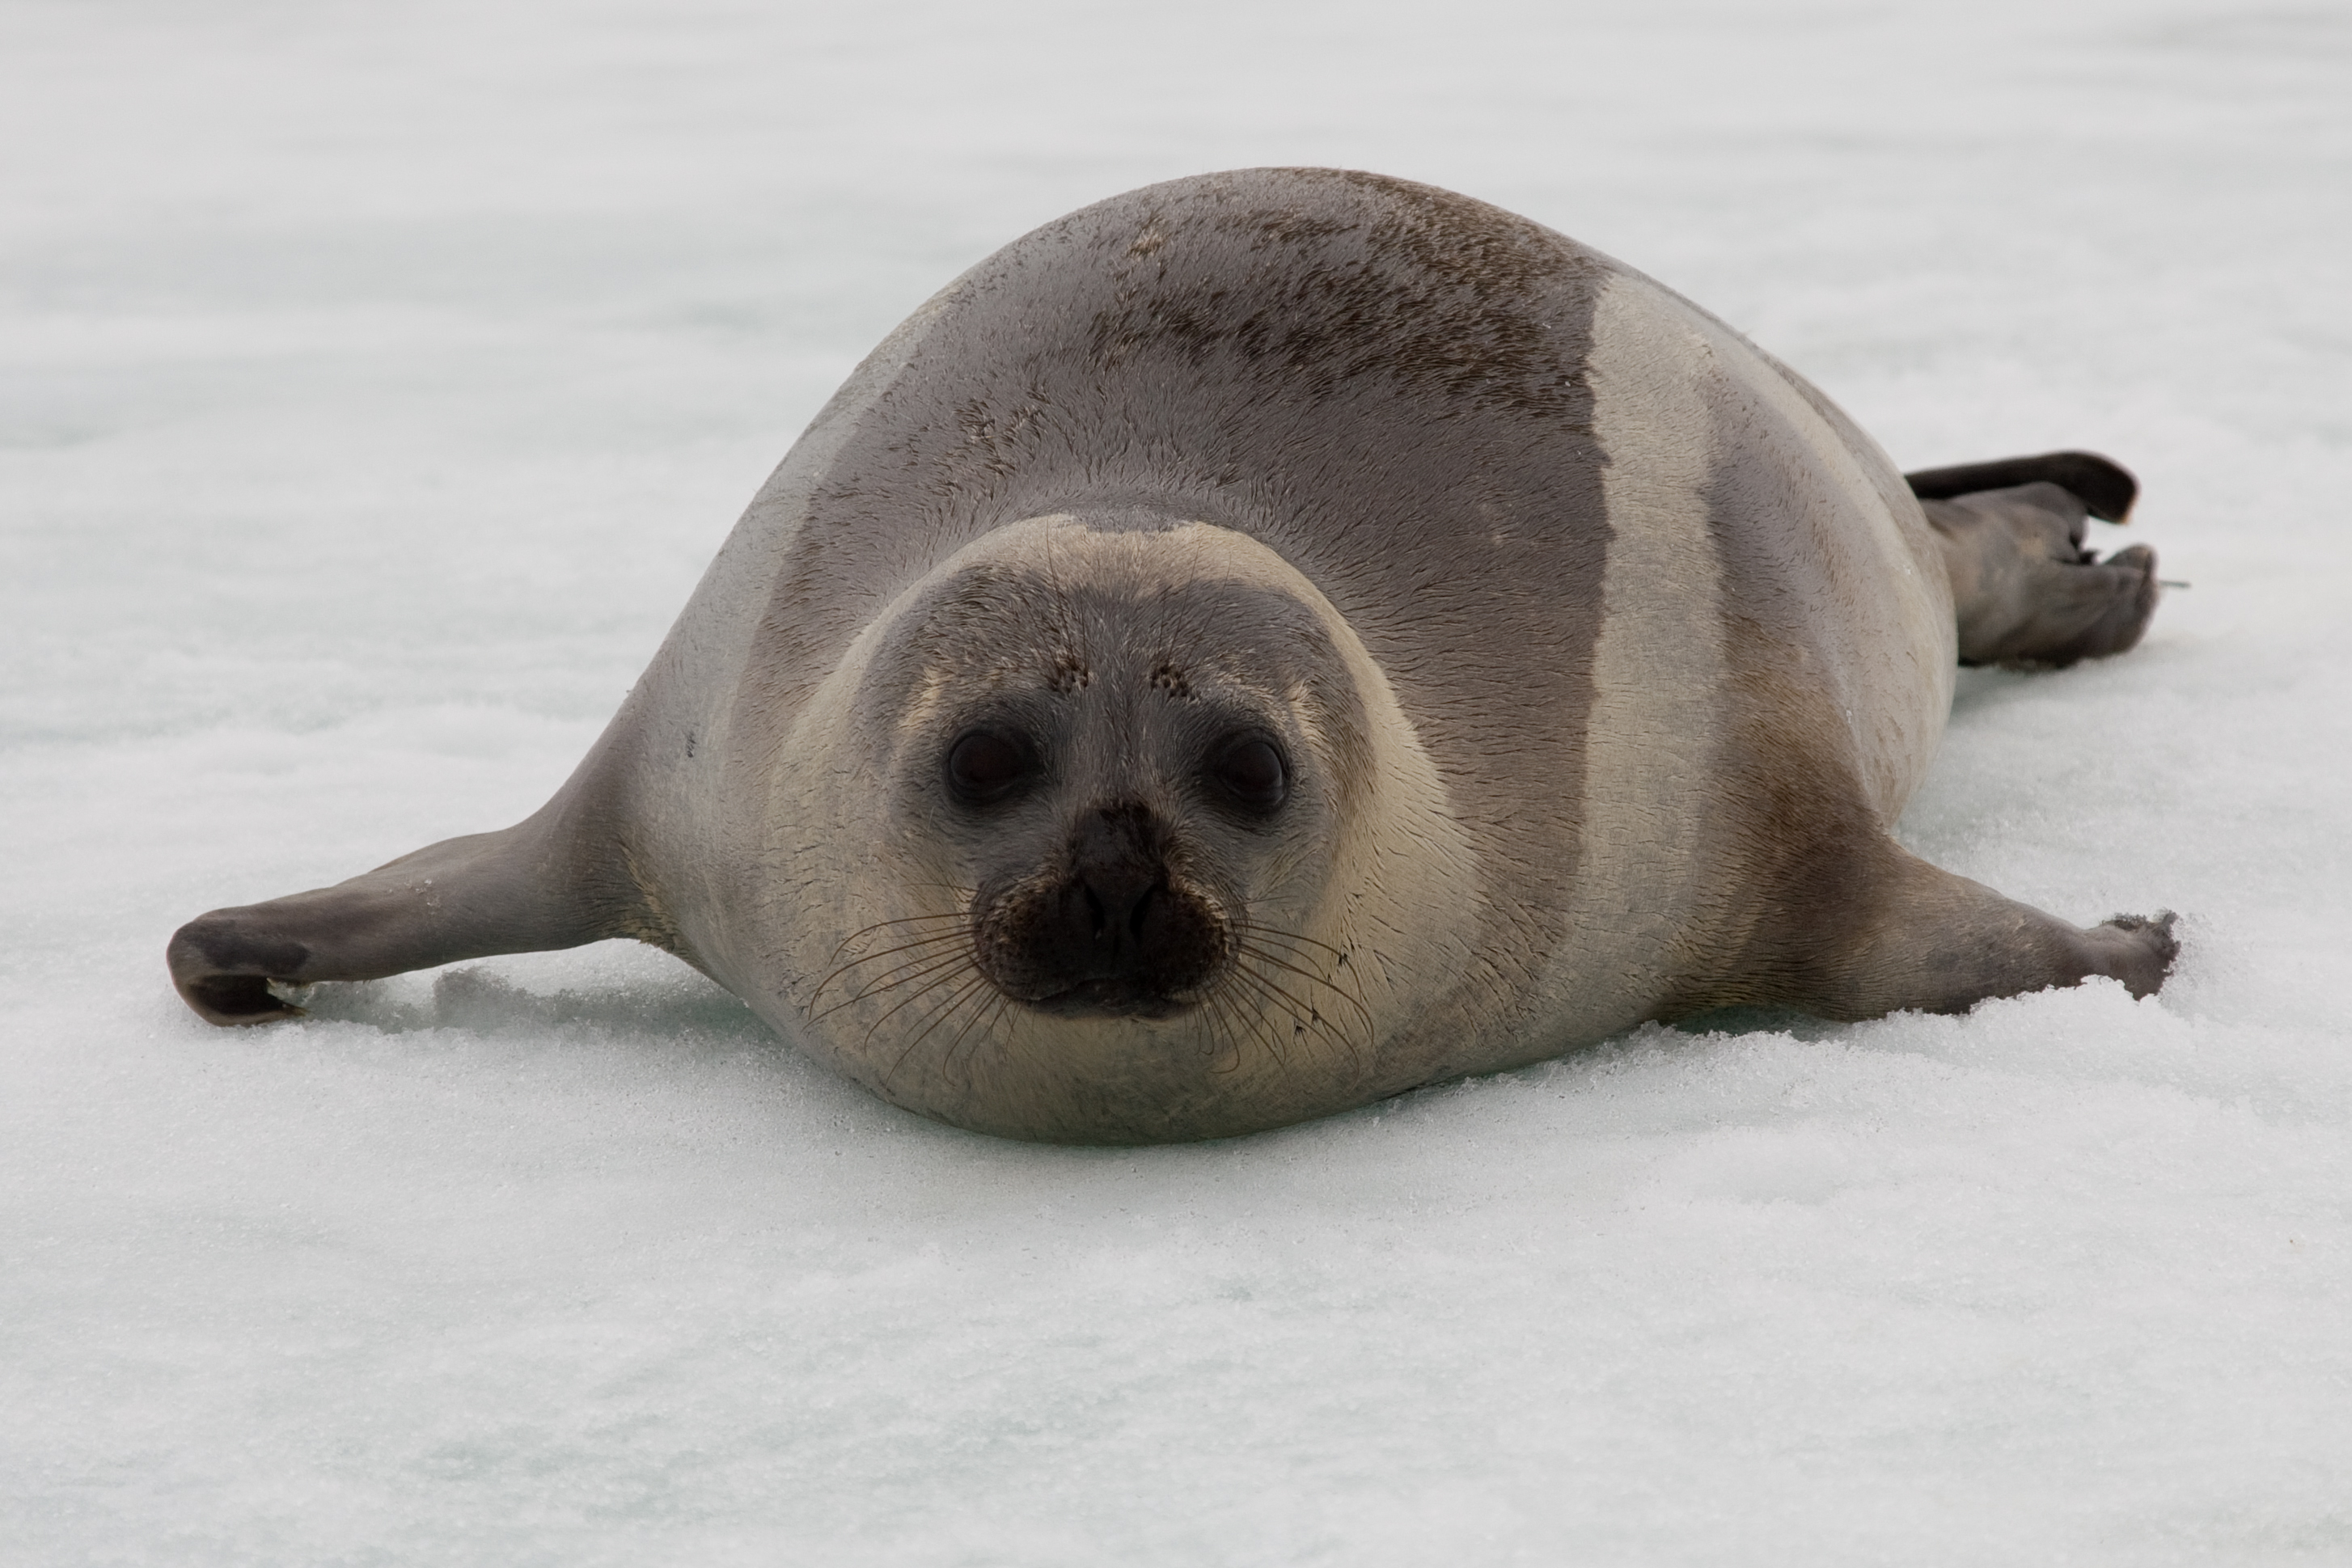
\includegraphics[width=6in]{ribbon}
%\end{center}
%\caption{ }
%\label{fig:ribbon}
%\end{figure}

\begin{figure}[!h]
\begin{center}
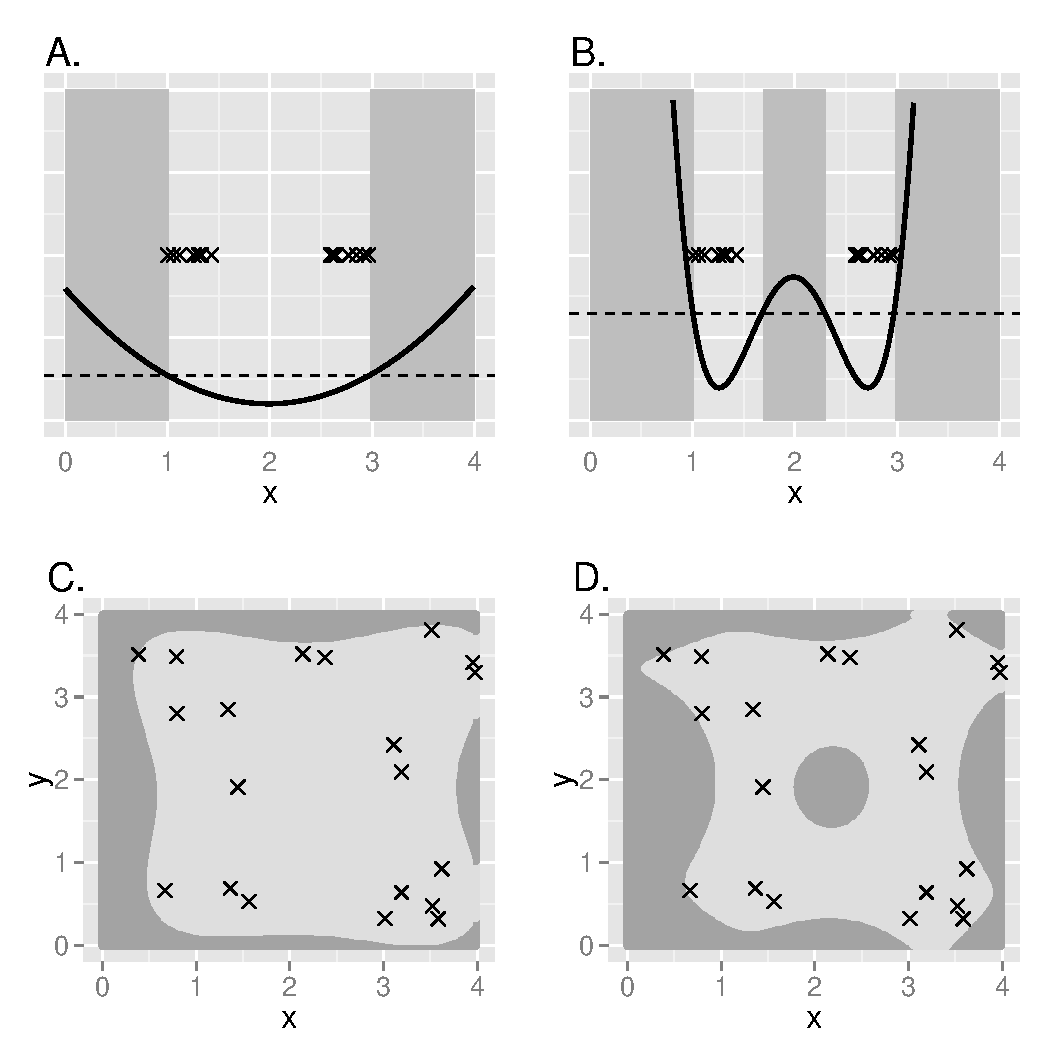
\includegraphics[width=6in]{IVH_simple2.pdf}
\end{center}
\caption{ }
\label{fig:IVH}
\end{figure}

\begin{figure}[!h]
\begin{center}
\includegraphics[width=6in]{BOSS_survey_ribbon.pdf}
\end{center}
\caption{ }
\label{fig:flights}
\end{figure}


\begin{figure}[!h]
\begin{center}
\includegraphics[width=6in]{ribbon_maps.pdf}
\end{center}
\caption{ }
\label{fig:ribbon_plot}
\end{figure}



\clearpage

\end{spacing}
\end{document} 